\documentclass[aspectratio=169,10pt]{beamer}
\usetheme[progressbar=frametitle,numbering=fraction,block=fill]{metropolis}
\usepackage{booktabs,amsmath,tabularx,multicol}
\usepackage{tikz}
\usepackage[siunitx]{circuitikz}
\usetikzlibrary{arrows.meta,positioning,calc,shapes.geometric}
\definecolor{kth}{RGB}{25,84,166}
\definecolor{kthl}{RGB}{98,152,210}
\definecolor{hs}{RGB}{200,70,50}
\definecolor{ls}{RGB}{50,100,190}
\definecolor{pri}{RGB}{60,140,80}
\setbeamercolor{frametitle}{bg=kth,fg=white}
\setbeamercolor{progress bar}{fg=kthl,bg=kth!20}
\setbeamercolor{title separator}{fg=kthl}
\setbeamercolor{alerted text}{fg=hs}
\graphicspath{{figs/}{../paper/figures/}{../gate-bump/figures/}{../gate-driver/figures/}{../pcb-fab/figures/}{../design-report-v2/figures/}}
\newcommand{\src}[1]{\vfill{\tiny\color{gray}#1}}
% decision box
\newcommand{\decision}[1]{\begin{block}{Decision}#1\end{block}}
% design-flow strip, #1 = active step
\newcommand{\flowstrip}[1]{%
\noindent\resizebox{\linewidth}{!}{\begin{tikzpicture}[font=\tiny,node distance=1.5mm,
  s/.style={draw,rounded corners=1.5pt,minimum height=5mm,text width=15mm,align=center,inner sep=1pt}]
\foreach \k/\t [count=\i] in {1/Inputs,2/Device,3/{Submodule\\voltage},4/{One device,\\one driver},5/{$n$ in\\parallel},6/{$f_\mathrm{sw}$,\\DC link},7/{Gate drive\\$\rightarrow$ block},8/{Two\\blocks},9/{Verify\\block},10/{Rev A\\board}} {
  \ifnum\k=#1 \node[s,fill=kth,text=white] (n\k) at (\i*16.8mm,0) {\t};
  \else \node[s,fill=kth!8] (n\k) at (\i*16.8mm,0) {\t}; \fi}
\foreach \a/\b in {1/2,2/3,3/4,4/5,5/6,6/7,7/8,8/9,9/10} \draw[-{Latex[length=1mm]}] (n\a) -- (n\b);
\end{tikzpicture}}\par\vspace{1mm}}

\title{GaN Building Block for a 1200\,V, 300\,kW Stacked Polyphase Bridge Inverter}
\subtitle{From design inputs to the Rev A board: a decision-driven design}
\author{Enes Ayaz}
\institute{KTH Royal Institute of Technology}
\date{October 2026}

\begin{document}
\maketitle

\begin{frame}{Design flow}
\centering
\flowstrip{0}
\vspace{3mm}

\footnotesize
\begin{tabularx}{\linewidth}{@{}clX@{}}
\toprule
1 & Design inputs & 1200\,V, 300\,kW, $M\le1.15$, PMSM $\Rightarrow$ phase current \\
2 & Device & survey 100--650\,V Si/GaN $\Rightarrow$ 100\,V GaN, EPC2361 \\
3 & Submodule voltage & $V_m + L\,di/dt \le 90$\,V with 0.5\,nH, even and integer $N$ $\Rightarrow$ 75\,V, $N=16$ \\
4 & One device, one driver & first-cut loop (copper + MLCC ESL), LTspice: overshoot, energies $\Rightarrow$ $\le$\,80\,A per device \\
5 & Devices in parallel & identical cells: loss, $T_j$ with a realistic $R_\mathrm{th}$, $V_\mathrm{DS}$ vs $n$ $\Rightarrow$ at least 4 per switch \\
6 & $f_\mathrm{sw}$, DC link & losses, MLCC count and current ripple vs $f_\mathrm{sw}$ $\Rightarrow$ 50\,kHz (machine to confirm) \\
7 & Gate drive & one driver for many devices breaks dynamic sharing $\Rightarrow$ one driver per two cells = building block \\
8 & Two blocks & block-to-block sharing and circulating current via the AC connection \\
9--10 & Verification, Rev A & Q3D parasitics, switching, losses, thermal, gate bump, board, measurements \\
\bottomrule
\end{tabularx}
\end{frame}

%==================================================================== 1
\section{1\quad Design inputs}
\begin{frame}{Design inputs}
\flowstrip{1}
\begin{columns}[T]
\column{0.5\textwidth}
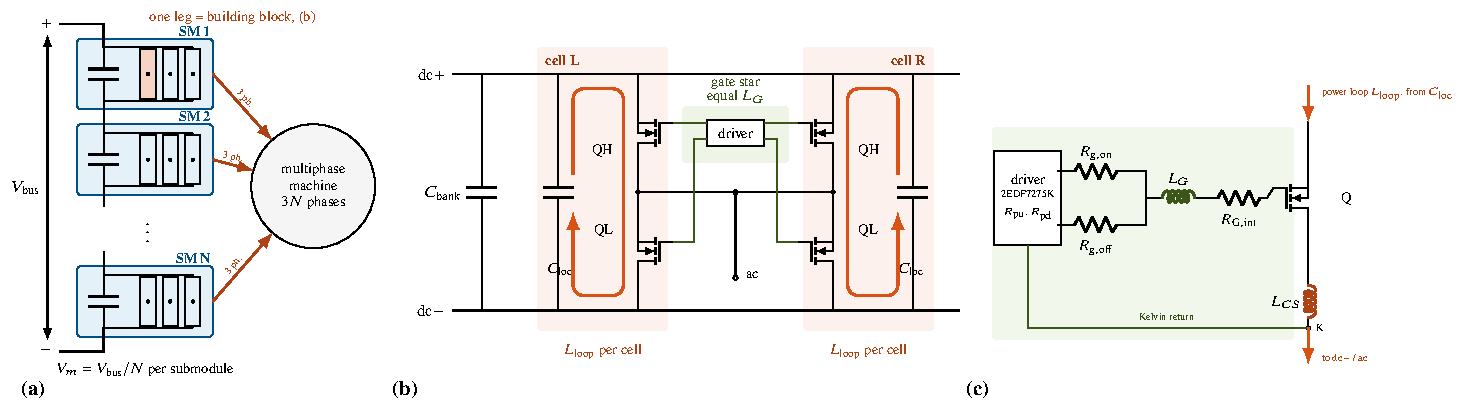
\includegraphics[width=\linewidth]{fig_spb_standalone.pdf}
\column{0.48\textwidth}
\small
\begin{tabular}{@{}ll@{}}
\toprule
DC bus & 1200\,V nominal \\
Output power & 300\,kW \\
Modulation index & $M \le 1.15$ (SVM) \\
Machine & PMSM, $\cos\varphi$ assumed 0.9 \\
Switching frequency & open (20--100\,kHz), step 6 \\
Coolant & 60\,$^\circ$C, $T_j \le 125\,^\circ$C \\
Device stress & $V_\mathrm{DS} \le 90$\,V at nominal bus (100\,V part) \\
\bottomrule
\end{tabular}

\vspace{1ex}
\footnotesize SPB: $N$ three-phase submodules in series on the DC side, each feeding one winding set; $V_m = 1200\,\mathrm{V}/N$.
\end{columns}
\end{frame}

\begin{frame}{Phase current follows from the inputs}
\flowstrip{1}
\vspace{1mm}
\begin{columns}[T]
\column{0.55\textwidth}
\small
Each of the $3N$ legs delivers $P/3N$ at the rms phase voltage $V_\mathrm{ph}=M V_m/(2\sqrt2)$:
\[
I_\mathrm{rms} = \frac{P}{3N\,V_\mathrm{ph}\cos\varphi}
 = \frac{P}{3\,\dfrac{M\,V_\mathrm{bus}}{2\sqrt2}\cos\varphi}
\]
\begin{itemize}
\item $N V_m = V_\mathrm{bus}$: the phase current does \alert{not} depend on $N$
\item $V_\mathrm{ph}$ = 1.15 $\cdot$ 75\,V/$2\sqrt2$ = 30.5\,V; 6.25\,kW per leg
\item \textbf{\IRMS\,A$_\mathrm{rms}$ per leg}, \IPK\,A peak ($\cos\varphi$ = 0.9)
\end{itemize}
\column{0.43\textwidth}
\small
\begin{tabular}{@{}cc@{}}
\toprule
$\cos\varphi$ & $I_\mathrm{rms}$ per leg \\
\midrule
1.00 & \IPFa\,A \\
0.95 & \IPFb\,A \\
0.90 & \textbf{\IPFc\,A} \\
0.85 & \IPFd\,A \\
\bottomrule
\end{tabular}

\vspace{1ex}
\footnotesize Losses below are for $\cos\varphi$ = 0.9; the PMSM operating point (field weakening, $\cos\varphi$) must be confirmed with the machine design.
\end{columns}
\end{frame}

%==================================================================== 2
\section{2\quad Device}
%%FRAME{Voltage class: why 100\,V GaN}
%%FRAME{EPC2361 key data}

%==================================================================== 3
\section{3\quad Submodule voltage}
\begin{frame}{Submodule voltage from $L\,di/dt$}
\flowstrip{3}
\begin{columns}[T]
\column{0.54\textwidth}
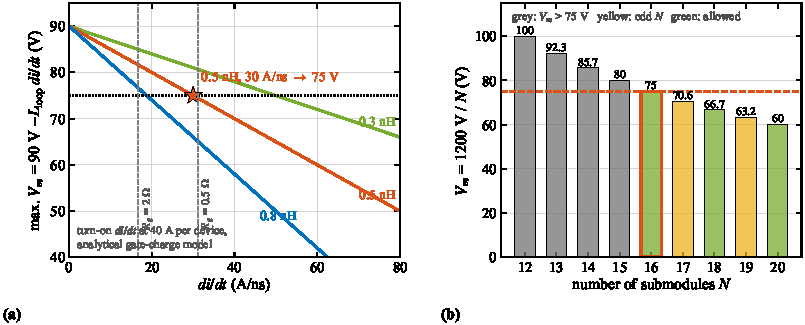
\includegraphics[width=\linewidth]{flow_vm.pdf}
\column{0.44\textwidth}
\scriptsize
\begin{itemize}
\item Peak stress $\hat v_\mathrm{DS} = V_m + L_\mathrm{loop}\,di/dt \le 90$\,V (10\,\% below the 100\,V rating)
\item First-cut loop with MLCCs: $L_\mathrm{loop}\approx$\,0.5\,nH per cell
\item To use the device fully we want fast switching: $\approx$\,30\,A/ns (analytical gate-charge model, 40\,A per device, $R_g$ 0.5--2\,$\Omega$) $\Rightarrow$ 15\,V overshoot
\item $\Rightarrow$ $V_m \le 75$\,V
\item $N$ must be an integer and even (symmetric arrangement of submodules and winding sets): 14 cells give 86\,V, 18 cells 67\,V and 12.5\,\% more parts
\end{itemize}
\decision{$V_m$ = 75\,V, $N$ = 16}
\end{columns}
\end{frame}

\begin{frame}{Why not lower: every submodule costs parts and loss}
\flowstrip{3}
\begin{columns}[T]
\column{0.5\textwidth}
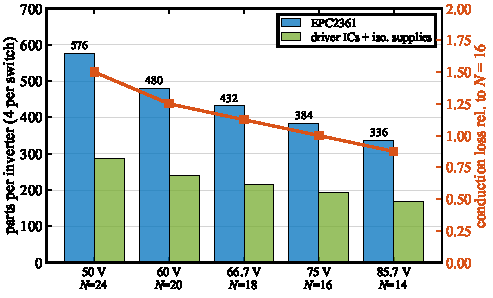
\includegraphics[width=\linewidth]{flow_cells.pdf}
\column{0.48\textwidth}
\small
\begin{itemize}
\item Phase current is fixed by $P$, $V_\mathrm{bus}$, $M$, $\cos\varphi$, not by $N$
\item Each submodule carries the full phase current $\Rightarrow$ conduction loss, transistors, drivers and isolated supplies all scale with $N$
\item 60\,V ($N$ = 20): +25\,\% parts and conduction loss
\item At the maximum bus voltage the overshoot margin shrinks; this is checked again with the final layout (Q3D, 0.374\,nH per cell)
\end{itemize}
\end{columns}
\end{frame}

%==================================================================== 4
\section{4\quad One device, one driver}
\begin{frame}{First-cut power loop of one cell}
\flowstrip{4}
\begin{columns}[T]
\column{0.54\textwidth}
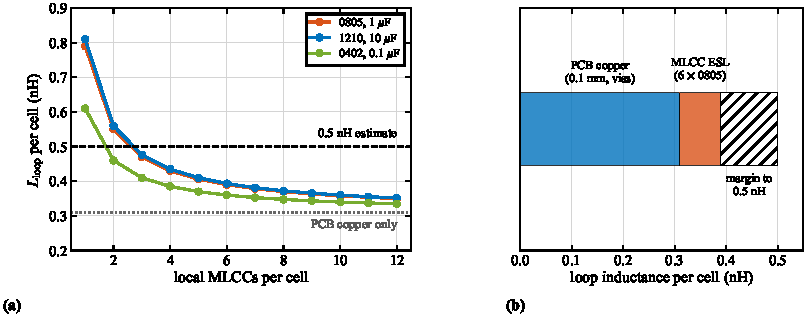
\includegraphics[width=\linewidth]{flow_loop.pdf}
\column{0.44\textwidth}
\scriptsize
\begin{itemize}
\item Loop = PCB copper (vertical loop over a 0.1\,mm dielectric, vias, pads) + ESL of the local MLCCs; the LGA package is in the device model
\item Copper alone $\approx$\,\LCU\,nH; MLCCs in parallel add ESL/$n_c$
\item 1 / 2 / 4 / 6 MLCCs: \LONE\ / \LTWO\ / \LFOUR\ / \LSIX\,nH: beyond $\approx$\,4 the number hardly matters
\item Chosen part: 1\,\textmu F 100\,V X7S 0805 (TDK C2012X7S2A105K125AB), next to the drains
\end{itemize}
\decision{Design with $L_\mathrm{loop}$ = 0.5\,nH per cell (0.3 and 0.8\,nH as bounds)}
\end{columns}
\end{frame}

\begin{frame}{One EPC2361 per switch: how fast and how much overshoot}
\flowstrip{4}
\centering
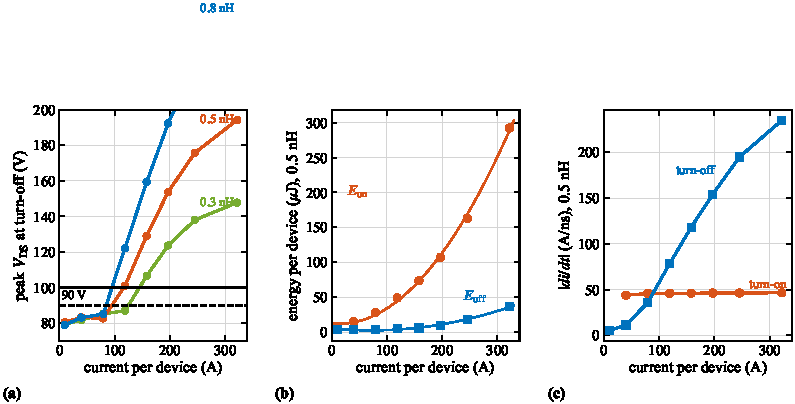
\includegraphics[width=\linewidth,height=0.37\textheight,keepaspectratio]{flow_single.pdf}
\footnotesize
\begin{itemize}
\item LTspice half bridge, double pulse at 75\,V: lumped loop, 1.7\,nH gate loop, 0.03\,nH common source, 2\,$\Omega$ on / 0\,$\Omega$ off, 4\,A/8\,A driver
\item Turn-on $di/dt$ is set by the driver ($\approx$\,45\,A/ns); turn-off $di/dt$ grows with current as the output capacitance charges faster
\item 0.5\,nH: \VLeighty\,V at \ILeighty\,A, \alert{\VLonetwenty\,V at \ILonetwenty\,A} per device; $E_\mathrm{on}$ grows quadratically
\item One device would carry \IPK\,A peak $\Rightarrow$ \textbf{current per device must stay $\le$\,80\,A}
\end{itemize}
\end{frame}

%==================================================================== 5
\section{5\quad Devices in parallel}
\begin{frame}{Thermal path per device}
\flowstrip{5}
\begin{columns}[T]
\column{0.55\textwidth}
\small
\begin{tabular}{@{}lr@{}}
\toprule
Layer (top-side cooling, per device) & K/W \\
\midrule
%%RTHTABLE
\midrule
Junction--coolant & \textbf{\RTH} \\
\bottomrule
\end{tabular}
\column{0.43\textwidth}
\small
\begin{itemize}
\item The earlier 2.1\,K/W was optimistic: two TIM layers and the cold plate dominate
\item Used for the decisions: \textbf{\RTH\,K/W}, coolant 60\,$^\circ$C
\item Bounds: 2.1\,K/W (sintered/soldered stack) and 8\,K/W (gap pad, as on the lab board)
\item $R_\mathrm{DS(on)}(T_j)$ from the datasheet curve (1.49 at 100\,$^\circ$C, 1.80 at 150\,$^\circ$C)
\end{itemize}
\end{columns}
\end{frame}

\begin{frame}{$n$ identical cells per switch (one device and one driver each)}
\flowstrip{5}
\centering
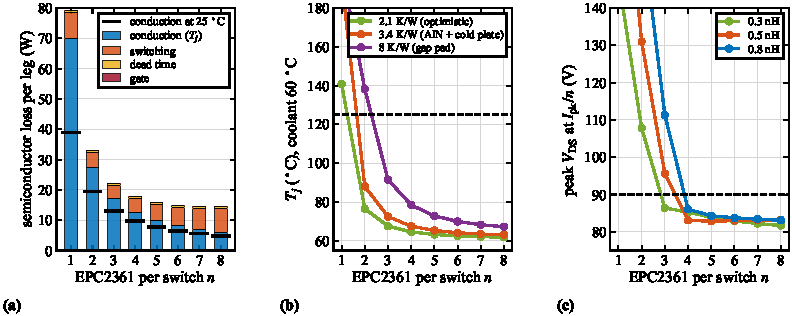
\includegraphics[width=\linewidth,height=0.42\textheight,keepaspectratio]{flow_npar.pdf}
\footnotesize
\begin{itemize}
\item \IRMS\,A$_\mathrm{rms}$ per leg, 50\,kHz, $T_j$ and $R_\mathrm{DS(on)}$ solved together; LTspice energies at 0.5\,nH
\item $n$ = 1: $T_j$ beyond 150\,$^\circ$C; $n$ = 2: \Pb\,W and \Vb\,V; $n$ = 3: \Vc\,V at 0.5\,nH
\item $n$ = 4 / 8: \Pd\,/\,\Ph\,W per leg; above 4 the gain is small while $E_\mathrm{oss}$ and drivers grow
\end{itemize}
\vspace{-1ex}
\decision{At least \textbf{4 EPC2361 per switch} ($V_\mathrm{DS}$ and $T_j$ for all three $R_\mathrm{th}$; 4 also splits into two equal pairs)}
\end{frame}

\begin{frame}{Where the loss comes from: line period and junction temperature}
\flowstrip{5}
\centering
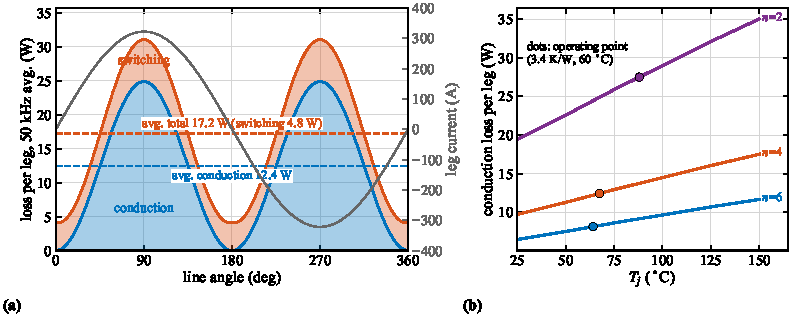
\includegraphics[width=\linewidth,height=0.48\textheight,keepaspectratio]{flow_wave.pdf}
\footnotesize
\begin{itemize}
\item $n$ = 4, 50\,kHz: switching loss follows $|i|$ (plus a constant $E_\mathrm{oss}$ part), conduction loss follows $i^2$; both peak at the current maximum
\item Conduction loss at the operating point is \CONDINC\,\% above its 25\,$^\circ$C value; with $n$ = 2 the self-heating loop ($T_j\uparrow\Rightarrow R_\mathrm{DS(on)}\uparrow$) is much stronger
\end{itemize}
\end{frame}

\begin{frame}{Losses vs number in parallel}
\flowstrip{5}
\footnotesize
\begin{tabular}{@{}lrrrrrrrr@{}}
\toprule
$n$ per switch & 1 & 2 & 3 & 4 & 5 & 6 & 7 & 8 \\
\midrule
%%NTABLE
\bottomrule
\end{tabular}

\vspace{1ex}
\footnotesize Semiconductor losses only (conduction at $T_j$, switching incl.\ $E_\mathrm{oss}$, dead time, gate), \RTH\,K/W, 60\,$^\circ$C coolant, 0.5\,nH, 50\,kHz. Board copper and MLCC losses are added for the block on the verification slides. Efficiency relative to 6.25\,kW per leg.
\end{frame}

%==================================================================== 6
\section{6\quad Switching frequency and DC link}
\begin{frame}{Switching frequency: losses, DC-link capacitors, current ripple}
\flowstrip{6}
\centering
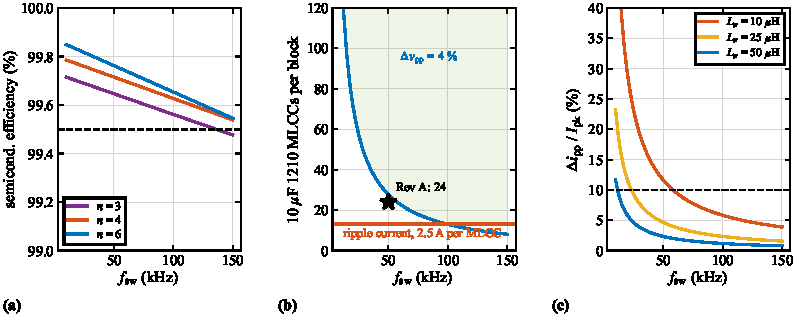
\includegraphics[width=\linewidth,height=0.34\textheight,keepaspectratio]{flow_fsw.pdf}
\scriptsize
\begin{itemize}
\item (a) $n$ = 4: \ETAtwenty\,/\,\ETAfifty\,/\,\ETAhundred\,\% at 20 / 50 / 100\,kHz
\item (b) DC link per block (\IBLK\,A$_\mathrm{rms}$, 4\,\% ripple, 10\,\textmu F 1210 at 30\,\% of $C$ at 75\,V): voltage ripple sets the count below $\approx$\,\FCROSS\,kHz, ripple current above; at 50\,kHz $\approx$\,\NVfifty\ MLCCs
\item (c) Winding current ripple $\Delta i_\mathrm{pp} = V_m/(4L_\sigma f_\mathrm{sw})$ depends on the machine leakage inductance $L_\sigma$ (not known yet)
\end{itemize}
\vspace{-1ex}
\decision{$f_\mathrm{sw}$ = 50\,kHz for the block design (efficiency and capacitor count balanced); final value with the machine ($L_\sigma$, iron loss)}
\end{frame}

\begin{frame}{Bypass capacitors: how many and how large}
\flowstrip{6}
\begin{columns}[T]
\column{0.44\textwidth}
\vspace{2mm}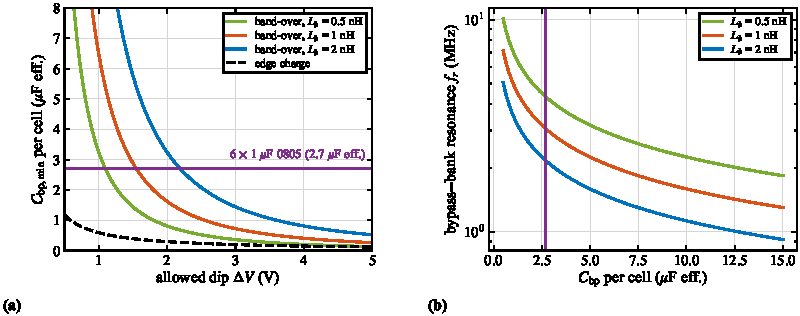
\includegraphics[width=\linewidth]{flow_bypass.pdf}
\column{0.54\textwidth}
\scriptsize
\textbf{Bypass} (1\,\textmu F 0805) supplies the edge, \textbf{bank} (10\,\textmu F 1210) the $f_\mathrm{sw}$ ripple. Per cell, \IDEV\,A:
\begin{enumerate}\setlength\itemsep{0pt}
\item \textbf{$di/dt$ $\rightarrow$ number}: $L_\mathrm{loop} = L_\mathrm{Cu} + \mathrm{ESL}/n \le 0.5$\,nH $\Rightarrow n \ge 4$
\item \textbf{Edge charge}: $\Delta Q = I(t_{ri}/2 + t_{vf}) + Q_\mathrm{oss}$, $t_{ri} = I/(di/dt)$ = \TRI\,ns, $t_{vf} = V/(dv/dt)$ = \TVF\,ns: \DQ\,\textmu C $\Rightarrow$ \CEDGE\,\textmu F for 1.5\,V ($C_\mathrm{oss}\,dv/dt$ = \IOSS\,A is included in $Q_\mathrm{oss}$)
\item \textbf{Hand-over to the bank} through $L_b$: $\Delta V \approx \Delta I\sqrt{L_b/C_\mathrm{bp}}$ $\Rightarrow$ $C_\mathrm{bp} \ge L_b(\Delta I/\Delta V)^2$ = \CHO\,\textmu F (1\,nH, 1.5\,V): \alert{sets the capacitance}
\item \textbf{Checks}: $C_\mathrm{bp} \gg C_\mathrm{oss}$ ($\ge$\,20$\times$); bypass--bank resonance $f_r$ = \FR\,MHz is excited every edge, damped only by ESR $\Rightarrow$ no more bypass than needed, $C_\mathrm{bank} \ge 10\,C_\mathrm{bp}$; X7S at 75\,V keeps 45\,\%
\end{enumerate}
\decision{6 $\times$ 1\,\textmu F 0805 per cell (2.7\,\textmu F eff.); $L_b$ to be extracted with Q3D on the routed board}
\end{columns}
\end{frame}

\begin{frame}{DC-link capacitor selection}
\flowstrip{6}
\begin{columns}[T]
\column{0.55\textwidth}
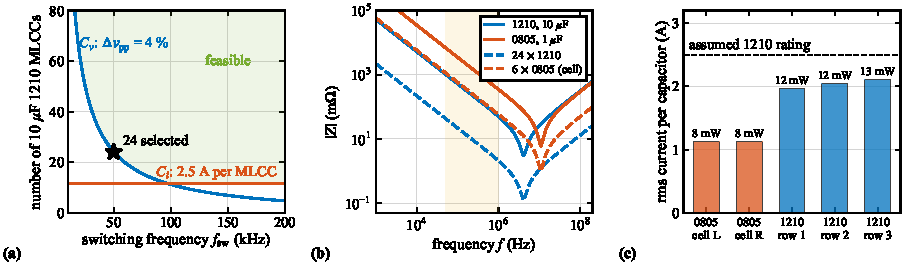
\includegraphics[width=\linewidth]{fig_dclink.pdf}
\column{0.43\textwidth}
\footnotesize
\begin{itemize}
\item Local: 6\,$\times$ 1\,\textmu F 0805 per cell (loop inductance, slide 4); bank: 10\,\textmu F 100\,V X7S 1210 (Murata GRM32EC72A106KE05L)
\item $C$ at 75\,V only $\approx$\,30\,\% of nominal (X7S DC bias)
\item Rev A has 24 per block, sized for 100\,A$_\mathrm{rms}$; at \IBLK\,A and 50\,kHz the ripple is $\approx$\,\DVREVA\,\% (4\,\% from \FREVA\,kHz), or add MLCCs in Rev B
\item Loss $\approx$\,0.4--0.5\,W per block; ripple current $\approx$\,2\,A per part
\end{itemize}
\end{columns}
\end{frame}
%==================================================================== 6
\section{7\quad Gate drive: from 4 devices to a building block}
\begin{frame}{Can one driver drive all four?}
\flowstrip{7}
\begin{columns}[T]
\column{0.58\textwidth}
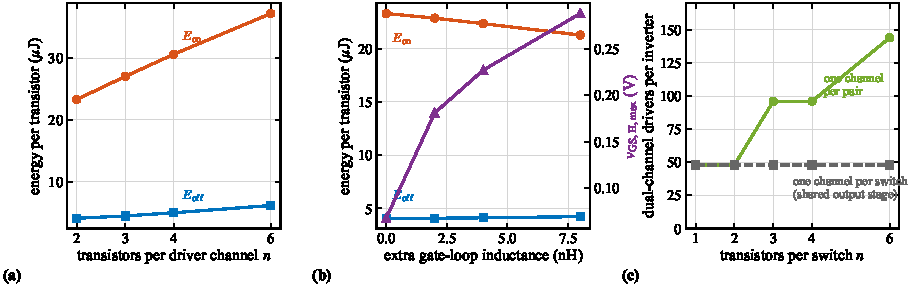
\includegraphics[width=\linewidth]{drv_scaling.pdf}
\column{0.4\textwidth}
\small
\begin{itemize}
\item One channel for 3 / 4 / 6 transistors: $E_\mathrm{on}$ per transistor $+16$ / $+31$ / $+60$\,\%
\item Peak sink current 12--14\,A, above the 8\,A rating
\item Longer gate tree brings the gate bump back
\item One driver per device: symmetric, but 4 channels and isolated supplies per switch
\end{itemize}
\end{columns}
\end{frame}
%%FRAME{Why symmetry: current-sharing sensitivity}
%%FRAME{Kelvin source on the EPC2361}

\begin{frame}{Building block: two mirrored cells, one centre driver}
\flowstrip{7}
\begin{columns}[T]
\column{0.5\textwidth}
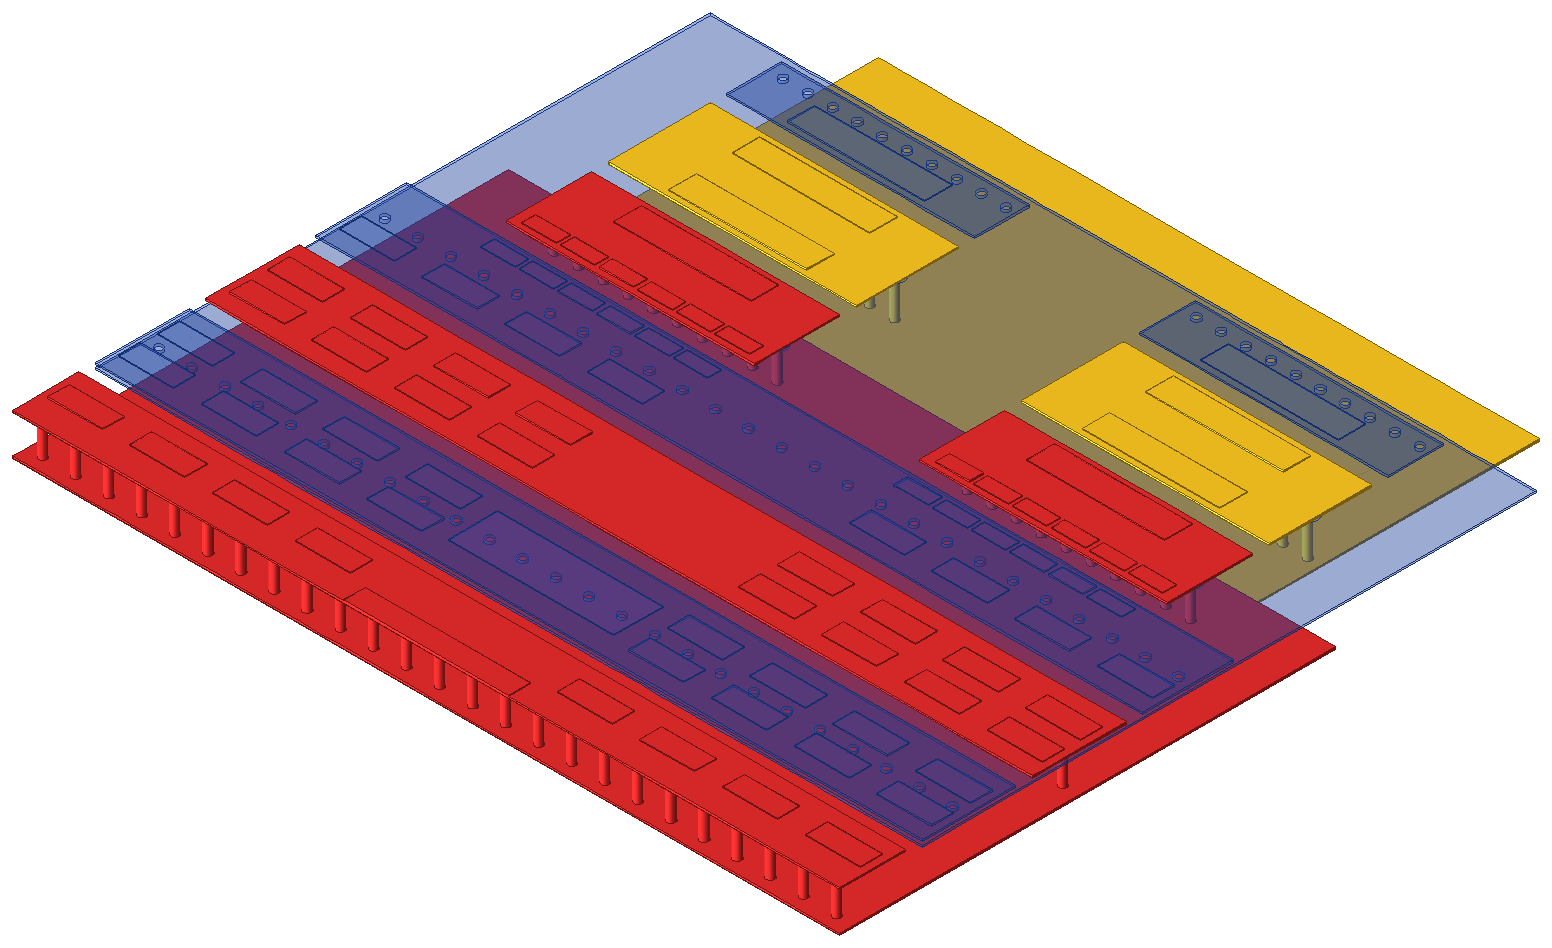
\includegraphics[width=\linewidth]{q3d_model.png}
\column{0.48\textwidth}
\small
\begin{itemize}
\item Two cells mirrored about the driver: identical gate loops and Kelvin returns for both transistors of a switch
\item One 2EDF7275K channel drives a \textbf{pair} symmetrically (star gate network)
\item Each cell keeps its own commutation loop (0.374\,nH per cell)
\end{itemize}
\decision{Building block = 2\,$\times$ EPC2361 per switch, one driver; \textbf{4 per switch = two blocks}}
\end{columns}
\end{frame}

%==================================================================== 7
\section{8\quad Two blocks in parallel}
\begin{frame}{Two building blocks per leg}
\flowstrip{8}
\begin{columns}[T]
\column{0.54\textwidth}
\centering
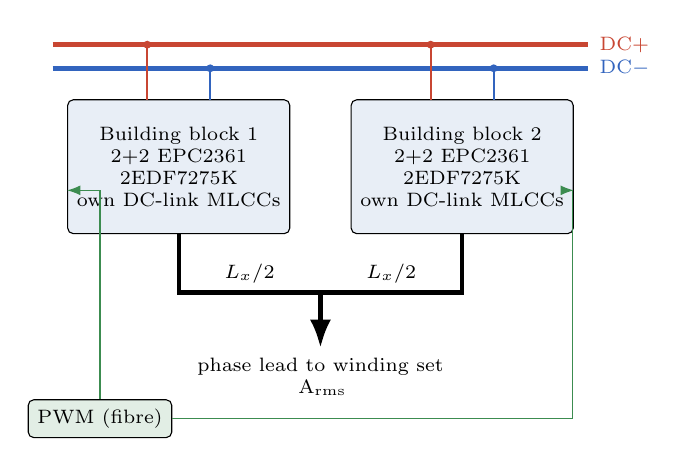
\begin{tikzpicture}[font=\scriptsize,
  blk/.style={draw,rounded corners=2pt,fill=kth!10,minimum width=24mm,minimum height=17mm,align=center}]
\node[blk] (a) at (0,0) {Building block 1\\2+2 EPC2361\\2EDF7275K\\own DC-link MLCCs};
\node[blk] (b) at (3.6,0) {Building block 2\\2+2 EPC2361\\2EDF7275K\\own DC-link MLCCs};
\draw[hs,line width=1.6pt] (-1.6,1.55) -- (5.2,1.55) node[right]{DC$+$};
\draw[ls,line width=1.6pt] (-1.6,1.25) -- (5.2,1.25) node[right]{DC$-$};
\foreach \x in {-0.4,3.2} {\draw[hs,thick] (\x,1.55) -- (\x,0.85); \fill[hs] (\x,1.55) circle (0.05);}
\foreach \x in {0.4,4.0} {\draw[ls,thick] (\x,1.25) -- (\x,0.85); \fill[ls] (\x,1.25) circle (0.05);}
\draw[line width=1.6pt] (0,-0.85) -- (0,-1.6) -- (3.6,-1.6) -- (3.6,-0.85);
\draw[line width=1.6pt,-{Latex}] (1.8,-1.6) -- (1.8,-2.3);
\node[below,align=center] at (1.8,-2.3) {phase lead to winding set\\\IRMS\,A$_\mathrm{rms}$};
\node[above] at (0.9,-1.6) {$L_x/2$};
\node[above] at (2.7,-1.6) {$L_x/2$};
\node[draw,fill=pri!15,rounded corners=2pt] (f) at (-1.0,-3.2) {PWM (fibre)};
\draw[pri,-{Latex}] (f.north) -- (-1.0,-0.3) -- (a.west|- 0,-0.3);
\draw[pri,-{Latex}] (f.east) -- (5.0,-3.2) -- (5.0,-0.3) -- (b.east|- 0,-0.3);
\end{tikzpicture}
\column{0.44\textwidth}
\small
\begin{itemize}
\item Two unchanged blocks share the submodule DC link and are joined at the AC side
\item Per block \IBLK\,A$_\mathrm{rms}$ (\IRMS\,A per leg)
\item Commutation stays inside each block (own MLCCs)
\item System: 96 blocks, 96 drivers, 384 EPC2361; series DC chain carries 250\,A
\end{itemize}
\end{columns}
\end{frame}

\begin{frame}{Sharing between blocks: driver skew and the AC connection}
\flowstrip{8}
\centering
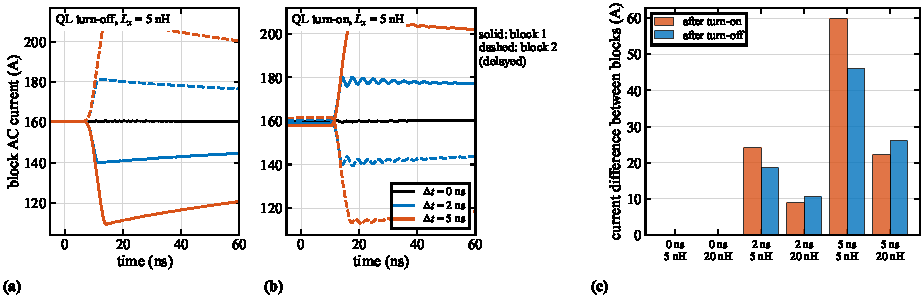
\includegraphics[width=\linewidth,height=0.40\textheight,keepaspectratio]{flow_twoblock.pdf}
\footnotesize
\begin{itemize}
\item LTspice, two complete blocks at \IPK\,A, PWM of block 2 delayed by $\Delta t$; $L_x$ = AC inductance between the switch nodes
\item At each edge the leading block takes $\Delta I \approx V_m\Delta t/L_x$ and keeps it until the next edge, where the sign reverses: a \alert{circulating current at $f_\mathrm{sw}$} through the AC connection
\item %%TWOTEXT
\end{itemize}
\end{frame}

\begin{frame}{Two blocks: requirements}
\flowstrip{8}
\small
\begin{columns}[T]
\column{0.5\textwidth}
\textbf{Static sharing}
\begin{itemize}
\item $R_\mathrm{DS(on)}$ has a positive temperature coefficient
\item Identical AC and DC connections (length, cross-section) for both blocks
\end{itemize}
\textbf{Dynamic sharing}
\begin{itemize}
\item One PWM receiver, fan-out to both drivers with matched traces
\item Driver skew $\le$\,2\,ns (2EDF7275K part-to-part delay from its datasheet still to be checked)
\item $L_x \gtrsim$\,20\,nH between the switch nodes (phase-lead geometry), not a stiff short bar
\end{itemize}
\column{0.48\textwidth}
\textbf{Verification}
\begin{itemize}
\item Double-pulse with both blocks: Rogowski on each block's AC lead (outside the commutation loop, so it fits)
\item Measure $\Delta I$ for a deliberately added delay, compare with LTspice
\item Continuous run: thermal camera on both blocks
\end{itemize}
\end{columns}
\end{frame}

%==================================================================== 8
\section{9\quad Verification of the building block}
\begin{frame}{Building block at the 300\,kW operating point}
\small
\begin{columns}[T]
\column{0.5\textwidth}
\begin{tabular}{@{}lr@{}}
\toprule
Current per block & \IBLK\,A$_\mathrm{rms}$ \\
Conduction ($T_j$) & \BCOND\,W \\
Switching + $E_\mathrm{oss}$ & \BSW\,W \\
Dead time + gate & \BDEAD\,W \\
Board copper (Q3D, incl.\ harmonics) & \BCU\,W \\
MLCCs & \BCAP\,W \\
\midrule
Total per block & \textbf{\BTOT\,W} \\
Efficiency (3.125\,kW per block) & \textbf{\BETA\,\%} \\
Per transistor / $T_j$ & \BPDEV\,W / \BTJ\,$^\circ$C \\
\bottomrule
\end{tabular}
\column{0.48\textwidth}
\begin{itemize}
\item Pair energies from the block LTspice model with the Q3D layout (one driver per pair), copper and MLCC losses scaled with $I^2$ from 100\,A; \RTH\,K/W, 60\,$^\circ$C coolant
\item $\cos\varphi$ = 1.0 / 0.85: \BTOTpfa\,/\,\BTOTpfd\,W per block
\item The following slides show the block analysis at its original 100\,A$_\mathrm{rms}$ design point (150\,kW with $M$ = 1.15, $\cos\varphi$ = 1)
\end{itemize}
\end{columns}
\end{frame}
%%FRAME{Extracted parasitics (Q3D)}
%%FRAME{Switching behaviour}
%%FRAME{Losses and efficiency}
%%FRAME{Thermal design}
%%FRAME{Gate bump at the high side}
%%FRAME{Mitigation: negative off-voltage}
%%FRAME{Driver: Infineon 2EDF7275K}
%%FRAME{Negative rail vs dead-time loss}
%%FRAME{Machine-integrated drive concept}
%%FRAME{Cell assembly and busbar}

%==================================================================== 9
\section{10\quad Rev A fabrication board}
%%FRAME{Rev A board: overview}
%%FRAME{Stack-up and design rules}
%%FRAME{Gate loops in the driver corridor}
%%FRAME{Separate turn-on and turn-off paths}
%%FRAME{Driver schematic (KiCad)}
%%FRAME{Isolated gate supplies}
%%FRAME{Supply schematic (KiCad)}
%%FRAME{Isolation domains}
%%FRAME{Double-pulse test: measurement landings}
%%FRAME{$E_\mathrm{on}$, $E_\mathrm{off}$ and per-transistor current}
%%FRAME{Bring-up: test points, LEDs, protection}
%%FRAME{Cooling for the load test}
%%FRAME{Power-stage schematic (KiCad)}

\section{Status and next steps}
%%FRAME{Verification status}
%%FRAME{Next steps}

\begin{frame}[standout]
Thank you\\[1ex]
\small Questions?
\end{frame}
\end{document}
